% !TeX root = ../tfg.tex
% !TeX encoding = utf8

\chapter{Experimentos Adicionales: Hiperparámetros}\label{ap:apendiceB}

En este apéndice se presentan dos experimentos relacionados con el uso de diferentes tamaños de \textit{batch} y \textit{learning rates} para un modelo que exhibe el DDD, con la finalidad de verificar su comportamiento ante distintas configuraciones. Para ello, se empleará la arquitectura $2$NN sobre el subconjunto MNIST[$4000/1000$], al cual se le añadirá un $10$\% de ruido, y sobre el que se probarán diversos tamaños de \textit{batch} y \textit{learning rates}.
 
\subsection*{Double descent con distinto tamaño de batch}

\begin{figure}[h!]
    \centering
    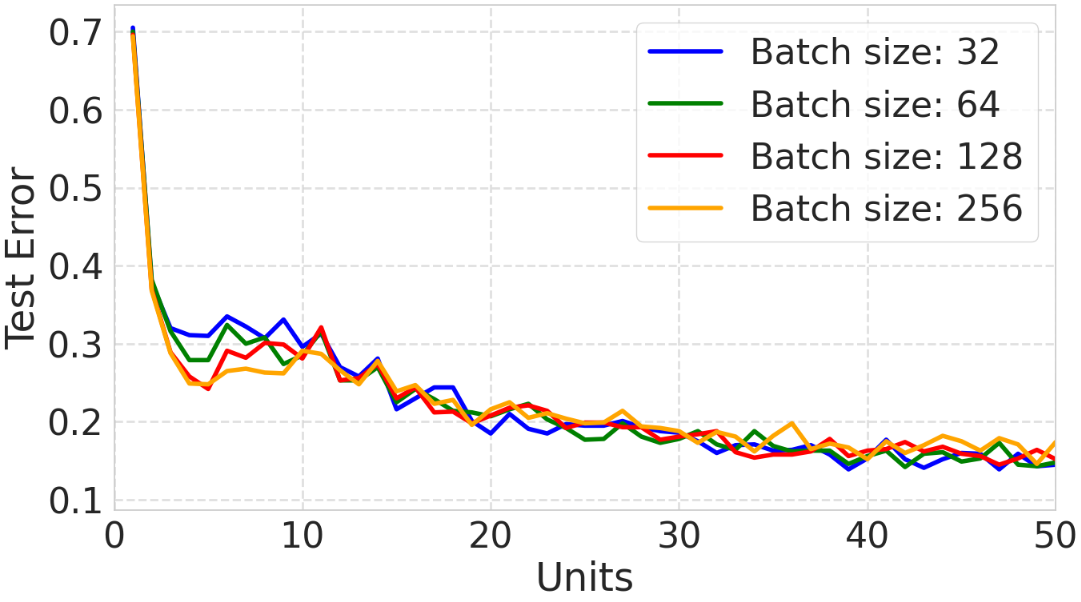
\includegraphics[width=0.65\textwidth]{img/experiments/batch_sizes_ddd.png}
    \caption[\textit{Deep Double Descent} para distintos tamaños de \textit{batch}.]{Error en test respecto a distintas configuraciones de tamaño de \textit{batch} de la red $2$NN sobre el subconjunto MNIST[$4000/1000$] con $10$\% de ruido añadido. Se observa el fenómeno bajo las diferentes configuraciones, destacando que, al emplear tamaños de \textit{batch} mayores, el error tiende a presentar menos oscilaciones.}\label{fig:dddbatchsizes}
\end{figure}

En la Figura~\ref{fig:dddbatchsizes} se observa que, para distintas configuraciones de tamaño de \textit{batch}, se manifiesta el \textit{Deep Double Descent}, siendo más notable (sin tantos altibajos en la curva del error) al utilizar tamaños mayores, debido a que se utiliza un mayor número de ejemplos para actualizar los parámetros en cada iteración. Por otro lado, la Tabla~\ref{tab:dddbatchsizes} muestra que, al incrementar el tamaño de \textit{batch}, el tiempo de entrenamiento disminuye, lo cual es lógico, ya que se procesan un mayor número de ejemplos en cada iteración. Por tanto, considerando ambos resultados, se concluye que utilizar un tamaño de \textit{batch} elevado ($128$ o $256$) es la opción adecuada para los distintos experimentos a realizar, ya que permite observar el fenómeno de forma más precisa y con menor coste computacional.

\begin{table}[h!]
    \centering
    \begin{tabular}{|c|c|c|c|}
    \hline
    \textbf{Modelo}       & \textbf{Dataset} & \textbf{Batch size} & \textbf{Entrenamiento} \\ 
    \hline
    $2$NN ($1-50$)     & MNIST[$4000/1000 - 10$\% noise]      & $32$      & $15$h $2$min         \\ 
    $2$NN ($1-50$)     & MNIST[$4000/1000 - 10$\% noise]      & $64$      & $11$h $56$min         \\ 
    $2$NN ($1-50$)     & MNIST[$4000/1000 - 10$\% noise]      & $128$      & $11$h $14$min         \\ 
    $2$NN ($1-50$)     & MNIST[$4000/1000 - 10$\% noise]      & $256$      & $10$h $23$min         \\
    \hline
    \end{tabular}
    \caption[Resumen de los experimentos realizados para el \textit{Deep Double Descent} con distinto tamaño de \textit{batch}.]{Resumen de los experimentos realizados para el \textit{Deep Double Descent} con distinto tamaño de \textit{batch} (\textit{batch size}).}\label{tab:dddbatchsizes}
\end{table}

\subsection*{Double descent con distinto learning rate}

\begin{figure}[h!]
    \centering
    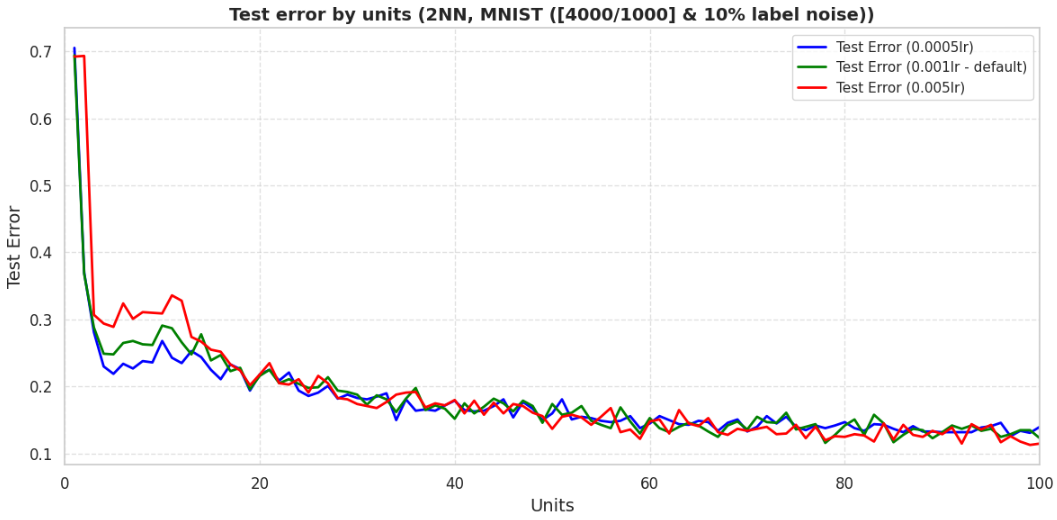
\includegraphics[width=0.65\textwidth]{img/experiments/learning_rates_ddd.png}
    \caption[\textit{Deep Double Descent} para distinto \textit{learning rate}.]{Error en test respecto a distintas configuraciones de \textit{learning rate} obtenido por la red $2$NN sobre el subconjunto MNIST[$4000/1000$] con $10$\% de ruido añadido. Se observa que, al utilizar valores más elevados para el \textit{learning rates}, el valor máximo del error es mayor.}\label{fig:difflr}
\end{figure}

En la Figura~\ref{fig:difflr} podemos observar cómo se manifiesta el DDD para distintas configuraciones de \textit{learning rate}. En particular, el pico del error de test se hace más pronunciado a medida que el \textit{learning rate} aumenta, dado que para un valor igual a $5 \times 10^{-4}$, el máximo error en test es mayor que para el valor por defecto del optimizador Adam ($10^{-4}$), y este, a su vez, es mayor que el máximo valor que proporciona el mínimo \textit{learning rate} utilizado ($5 \times 10^{-5}$).

En conclusión, esto nos indica que, si un modelo presenta el \textit{Deep Double Descent}, no es necesario preocuparse en exceso por ajustar de manera precisa el \textit{learning rate}, puesto que, dentro de ciertos rangos de valores de este hiperparámetro, el comportamiento característico del fenómeno se mantiene, lo que indica que el valor por defecto del mismo resulta ser suficiente para observar y estudiar dicho comportamiento sin afectar significativamente los resultados, lo que contribuye a simplificar el proceso de diseño experimental.

Finalmente, para concluir esta subsección, se muestra en la Tabla~\ref{tab:difflr} un resumen de los experimentos realizados, junto con sus respectivos tiempos de entrenamiento. Cabe destacar que el uso de distintos \textit{learning rates} no altera significativamente el tiempo de entrenamiento, dado que en todos los casos se realiza el mismo número de iteraciones.

\begin{table}[h!]
    \centering
    \begin{tabular}{|c|c|c|c|}
    \hline
    \textbf{Modelo}       & \textbf{Dataset} & \textbf{Learning rate} & \textbf{Entrenamiento} \\ 
    \hline
    $2$NN ($1-100$)     & MNIST[$4000/1000 - 10$\% noise]      & $0.005$      & $26$h $23$min   \\ 
    $2$NN ($1-100$)     & MNIST[$4000/1000 - 10$\% noise]      & $0.001$ (\textit{default})      & $26$h $50$min     \\ 
    $2$NN ($1-100$)     & MNIST[$4000/1000 - 10$\% noise]      & $0.0005$      & $27$h $2$min         \\ 
    \hline
    \end{tabular}
    \caption[Resumen de los experimentos realizados para el DDD con distinto \textit{learning rate}.]{Resumen de los experimentos realizados para el DDD con distinto \textit{learning rate}.}\label{tab:difflr}
\end{table}

\endinput
%------------------------------------------------------------------------------------
% FIN DEL APÉNDICE. 
%------------------------------------------------------------------------------------
